
\section{Experimental Setup} \label{sec:exp-setup}
\subsection{Predator vs Prey}
	The predator vs prey game consists of two types of agents (predators and prey) competing on a nine by nine board. The goal of the predator is to capture the prey and the goal of the prey is to avoid the predator for the 20 turns.  Both the predator and prey move simultaneously in this implementation. This should cause both the predators and the prey to learn to predict the movement patterns of their opponent .
	
\subsubsection{Predator}
  As stated before, the goal of the predator is to catch the prey. In order to interact with the environment, the predator has a neural network that is associated with it. This neural network’s input layer consists of 81 input nodes which read the 9 by 9 board state. There is a certain number of hidden nodes that was varied between runs, and there are 7 output nodes. The output node actions are arranged as seen in Table \ref{tab:pred-actions}. Some output nodes in the neural network are connected. These nodes are listed together in the table, and when the action for the set is decided, the node with the higher activation is used. The predator has two unique output nodes that the prey does not have access to. These output nodes apply a two times multiplier to the movement in either the horizontal or vertical direction. This could be thought of similar to a jump or pounce action from the predator's point of view. If there is no diagonal movement, then the largest of the 2, 3, 4 and 5 nodes will be taken to determine the direction of the movement.
				
\begin{table}
  \centering
  \begin{tabular}{|c|c|}
    \hline
    Output Node & Action \\
    \hline
    1 & Move diagonally (yes or no)\\
    2 and 3 & Horizontal movement left or right \\
    4 and 5 & Vertical movement up or down \\
    6 & Chase horizontally \\
    7 & Chase vertically \\
    \hline
  \end{tabular}
  \caption{Predator output node to action mapping}
  \label{tab:pred-actions}
\end{table}

\subsubsection{Prey}
  The actions of the prey are set up similarly to the actions of the predator. However the prey have a slightly smaller neural network. The prey neural network consists of the same 81 input nodes which accept the board state, followed by a certain number of hidden nodes that was varied between runs. Unlike the predators, they only have 5 output nodes. The actions that the prey can perform are summarized in Table \ref{tab:prey-actions}. The prey's neural network is similar to the predator's, except without the special nodes. For node set of 2 and 3, and set 4 and 5, the node with the higher activation is taken. If there is no diagonal movement, then the largest of the 2, 3, 4 and 5 nodes will be taken to determine the direction of the movement.

\begin{table}
  \centering
  \begin{tabular}{|c|c|}
    \hline
    Output Node & Action \\
    \hline
    1 & Move diagonally (yes or no)\\
    2 and 3 & Horizontal movement left or right \\
    4 and 5 & Vertical movement up or down \\
    \hline
  \end{tabular}
  \caption{Prey output node to action mapping}
  \label{tab:prey-actions}
\end{table}


	
\subsubsection{Game Progression}
		As the game is played and the learning of both the predator and prey progresses, some large gains and falls in fitness should be observed as one type of agent outsmarts the other and vice versa. The runs are expected to reach an equilibrium when averaged over time. 

\subsection{NN Implementation} 
	On an implementation level, the neural networks were implemented using an array of matrices which are multiplied together to calculate the output of the network. Each matrix represents the connection weights between 2 layers of the neural network. To accomplish this matrix representation, the RealMatrix library provided by \cite{apache} was used. The activation function utilized by all the nodes in the neural network was the logistic function. The weights of the connections (represented by the matrix) was evolved using particle swarm optimization.
	
\subsection{PSO Implementation}

\subsubsection{Particle Representation}
As the PSO is used to evolve the neural network, a particle representation of the neural network weights must be created. This was accomplished by using the weight values in the neural net matrices as the position of the particle. This results in a high dimensional particle where the dimensionality of the particle is equal to the number of connection in the neural network. Since the representation of the weights in the neural network is one-to-one to the location of the particle, as the particle location changes and updates the weights of the network are also updated.


\subsubsection{Calculating Fitness Values} \label{sec:calc-fitness}
Fitness values for particles are calculated by instructing each particle to play 400 games against particles from the other swarm. There were three different point systems that were experimented with. These are outlined in Table \ref{tab:game-rules}. The fitness value calculated was divided by the number of games that was played by the particle in order to reduce it to a range between -2 and +1. As seem in Table \ref{tab:game-rules}, game V1 is heavily stacked in favour of the prey as if the prey or predator fall off then the predator does not capture the prey and the prey gains a point. Game V2 is a balanced match between the two types of agents while game V3 provides a slight advantage to the prey because if the prey falls off then the predator loses one point, while if the predator falls off then the prey gains one point as it successfully avoided the predator.

\begin{table}
  \centering
  \begin{tabular}{|c|c|c|c|}
    \hline
    Game Version & Scenario & Predator Score & Prey Score\\
    \hline
    \multirow{ 5}{*}{V1} & Predator catches prey & +1 & -1 \\
    & Prey avoids predator & -1 & +1\\ 
    & Predator and prey fall & 0 & +1 \\
    & Predator falls & 0 & +1 \\
    & Prey falls & 0 & +1 \\
    \hline
    \multirow{ 5}{*}{V2} & Predator catches prey& +1 & -1\\
    & Prey avoids predator & -1 & +1\\ 
    & Predator and prey fall & -2 & -2 \\
    & Predator falls & -2 & 0 \\
    & Prey falls & 0 & -2 \\
    \hline
    \multirow{ 5}{*}{V3} &  Predator catches prey & +1 & -1\\
    & Prey avoids predator & -1 & +1\\
    & Predator and prey fall & -2 & -2\\
    & Predator falls, prey does not fall & -2 & +1 \\
    & Predator does not fall, prey falls & -1 & -2 \\
    \hline
  \end{tabular}
  \caption{Game Rules}
  \label{tab:game-rules}
\end{table}

\subsubsection{Simulation}
To set up the simulation, an opponent is selected randomly from the opposing swarm. The predator and prey are then placed on the board randomly such that the predator is on the upper half of the board and the prey is on the lower half of the board. Each turn consists of the predator and prey taking in the board surroundings and then deciding a move to make. The predator and prey then simultaneously make moves for 20 turns. The game ends if the predator catches the prey, or if the 20 turns have been made. 

\subsubsection{Board Encoding}
As mentioned, the neural network takes as input the board. Therefore, the board has to be encoded before it is given to the network. This board encoding encodes the 9x9 board as seen in Table \ref{tab:board-encoding-table}.

\begin{table}
  \centering
  \begin{tabular}{|c|c|}
    \hline
    Board State & Encoding \\
    \hline
    Empty Square & 0 \\
    Same Species & 1 \\
    Opposite Species & -1\\
   \hline
  \end{tabular}
  \caption{Game Board Encodings}
  \label{tab:board-encoding-table}
\end{table}

\subsubsection{Hall of Fame}
Both the predator and prey swarm have their own hall of fame which stores prior global best values of that swarm in order to provide some backtracking over time to see if a previous set of weights is more efficient than the current best weights. Each hall of fame can hold a maximum of 25 fitness values. The fitness values stored were the last 25 global best fitness values. The hall of fame is updated every time a new global best fitness is determined and the new global best weight value is stored in the hall of fame. The values in the hall of fame are re-run every 10 epochs in order to determine if any older values have a better fitness than the current best as these could change as the opponent swarm improves.

\subsection{Visual Board Representation}
In order to visualize the games played by the predator and prey agents, a visual board representation was developed. The representation consists of a nine by nine grid with two agents placed onto it. The predator agent is represented by a red circle, while the prey agent is represented by a green circle. The starting location of both agents are left unmarked, however a line is drawn between the old location and the next location that the agent moved to. Therefore, the tile with a line connecting to it without a circle is the starting tile. A labeled example of a game can be seen in Figure \ref{fig:label-game-example}.


\begin{figure}
  \centering
  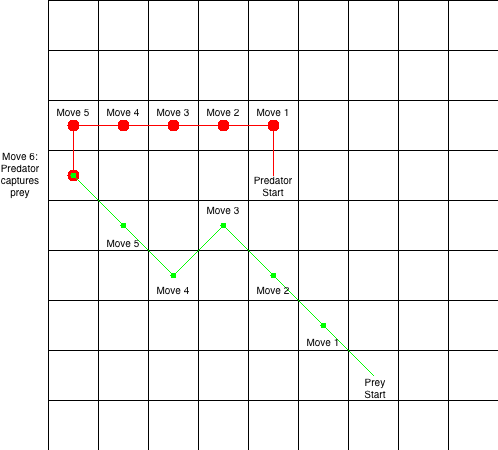
\includegraphics[width=0.7\textwidth]{Board-Visualization.png}
  \caption{Labeled visualization of the game board}
  \label{fig:label-game-example}
\end{figure}

\subsection{Run Summary}
Table \ref{tab:experiment-labels-1} contains all of the parameter sets that were tested. Throughout the experiments, the percentage of charged particles, core radius and perception limit combination, and number of hidden nodes were varied. The ability to fall off the board was also changed in order to see if any behavioural changes would develop. All charged particles had a charge value of 16. If a closer look at the game rules is taken, then it can be seen that if the ability to fall off is removed, then all three game rules simplify to the same values. In other words, if the predator catches the prey, then the predator gains one point while the prey loses a point. If the prey avoids the predator, then the opposite takes place. When discussing the results, the game rules version number will be prepended to the experiment number excluding when the agents cannot fall off the board. For each of the parameter sets, 5 runs we conducted. Each run consisted of 50 predators and 50 prey grouped into two swarms (one per agent type), being evolved over 500 iterations. Each game that way played took place over 20 turns unless the predator caught the prey, or either the predator or the prey fell off of the board.

\begin{table}
  \centering
  \begin{tabular}{|c|c|c|c|c|}
    \hline
    Experiment & Hidden Nodes & Core Radius & Perception Limit & Swarm Charged (\%) \\
    \hline
    1 & \multirow{ 8}{*}{15}  & \multirow{ 4}{*}{2} & \multirow{ 4}{*}{40} & 0 \\
    2 & & & & 33\\
    3 & & & & 67\\
    4 & & & & 100\\ \cline{3-5}
    5 & & \multirow{ 4}{*}{5} & \multirow{ 4}{*}{30} & 0 \\
    6 & & & & 33\\
    7 & & & & 67\\
    8 & & & & 100\\ \cline{2-5}
    9 & \multirow{ 8}{*}{30}  & \multirow{ 4}{*}{2} & \multirow{ 4}{*}{40} & 0 \\
    10 & & & & 33\\
    11 & & & & 67\\
    12 & & & & 100\\ \cline{3-5}
    13 & & \multirow{ 4}{*}{5} & \multirow{ 4}{*}{30} & 0 \\
    14 & & & & 33\\
    15 & & & & 67\\
    16 & & & & 100\\ \cline{2-5}
    17 & \multirow{ 8}{*}{60}  & \multirow{ 4}{*}{2} & \multirow{ 4}{*}{40} & 0 \\
    18 & & & & 33\\
    19 & & & & 67\\
    20 & & & & 100\\ \cline{3-5}
    21 & & \multirow{ 4}{*}{5} & \multirow{ 4}{*}{30} & 0 \\
    22 & & & & 33\\
    23 & & & & 67\\
    24 & & & & 100\\
    \hline
  \end{tabular}
  \caption{Experiment Summary}
  \label{tab:experiment-labels-1}
\end{table}